% !TeX root = ../../thesis.tex

The data was gathered from 9 different Portuguese hospitals regarding obstetric information: data from the mother, several data points about the fetus and delivery mode. The data is from 2019 to 2020. The software for collecting data was the same in every institution, and the columns were the same, even though the version of each software differed across hospitals. Across the different hospitals, data rows ranged from 2364 to 18177. The sum of all rows is 73351 rows. The data dictionary is in appendix A. This study received Institutional Review Board approval from all hospitals included in this study with the following references: Centro Hospitalar São João; 08/2021, Centro Hospitalar Baixo Vouga; 12-03-2021, Unidade Local de Saúde de Matosinho; 39/CES/JAS, Hospital da Senhora da Oliveira; 85/2020, Centro Hosptilar Tamega Sousa; 43/2020, Centro Hospitalar Vila Nova de Gaia/Espinho; 192/2020,Centro Hospitalar entre Douro e Vouga; CA-371/2020-0t\_MP/CC, Unidade Local de sa\'{u}de do Alto Minho; 11/2021. All methods were carried out in accordance with relevant guidelines and regulations. Data was anonymized before usage.

For this purpose, we took the Khan harmonized framework since we understood it as simpler to communicate we feel that the three main categories are indeed non-reducible, which makes sense from an organizational standpoint. Furthermore, the work done by Khan et al. with mapping to already existing frameworks could help compare this work with others who felt the need to use other frameworks. With this in mind, we will use three main categories, Completeness, Plausibility and Conformance. Completeness relates to missing data. Plausibility relates to how believable the values are. Conformance relates to the compliance of the data representation, like formatting, computational conformance and other data standards implemented. 

With this in mind, we will use three main categories, Completeness, Conformance and Plausibility. Completeness relates to missing data. Conformance relates to the compliance of the data representation, like formatting, computational conformance and other data standards implemented. Plausibility relates to how believable the values are.

%TC:ignore
\begin{figure}[htbp]
\centering
\caption{Dimensions of data quality}\label{fig:categories} 
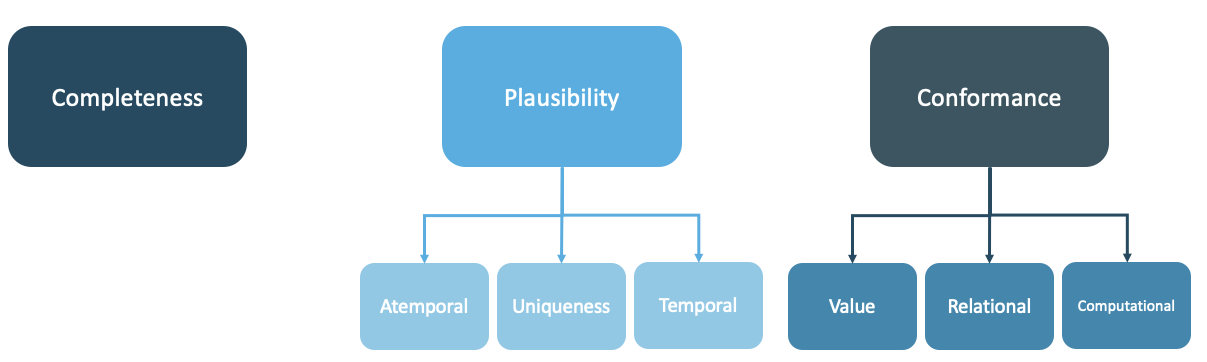
\includegraphics[scale=0.29]{figures/data-quality-v1.png}
\end{figure}
%TC:endignoregrama